\appendix
\pagenumbering{Roman}
\thispagestyle{empty}  
\renewcommand{\appendixname}{Appendix}%%přílohy, číslování římskými


\chapter*{Appendix A - \code{PyNfSA}: User Manual} 
\addcontentsline{toc}{chapter}{Appendix A - \code{PyNfSA}: User Manual}




\chapter*{Appendix B } 
\addcontentsline{toc}{chapter}{Appendix B}


%\section*{} 

%
%\section*{GARBAGE}
%
%\begin{figure}[h!]%
%  \centering
%  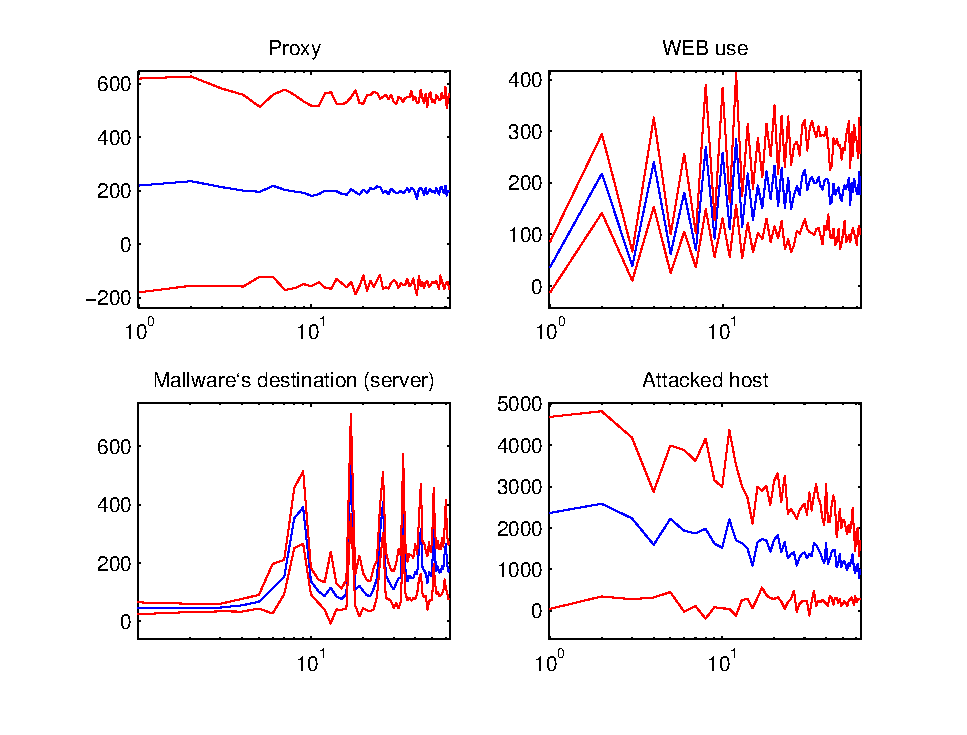
\includegraphics[width=140mm]{img/spect_dst_bdivp}
%  \caption{Spectrums ($mean$ - blue, $mean\pm st.dev$ - red) of some  endpoints using feature $r_t^{(1)}$ and agregation over \textbf{target}}
%  \label{fig:spect_dst_bdivp}
%\end{figure}
%\begin{figure}[h!]%
%  \centering
%  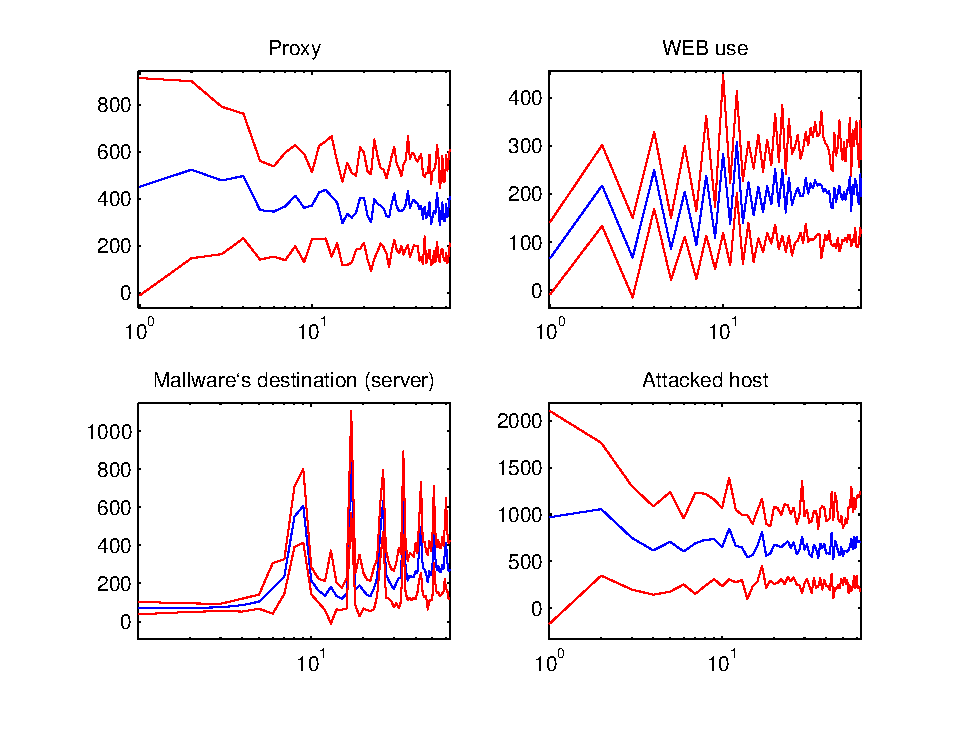
\includegraphics[width=140mm]{img/spect_src_bdivp}
%  \caption{Spectrums ($mean$ - blue, $mean\pm st.dev$ - red) of some  endpoints using feature $r_t^{(1)}$ and agregation over \textbf{source}}
%  \label{fig:spect_src_bdivp}
%\end{figure}
%\begin{figure}[h!]%
%  \centering
%  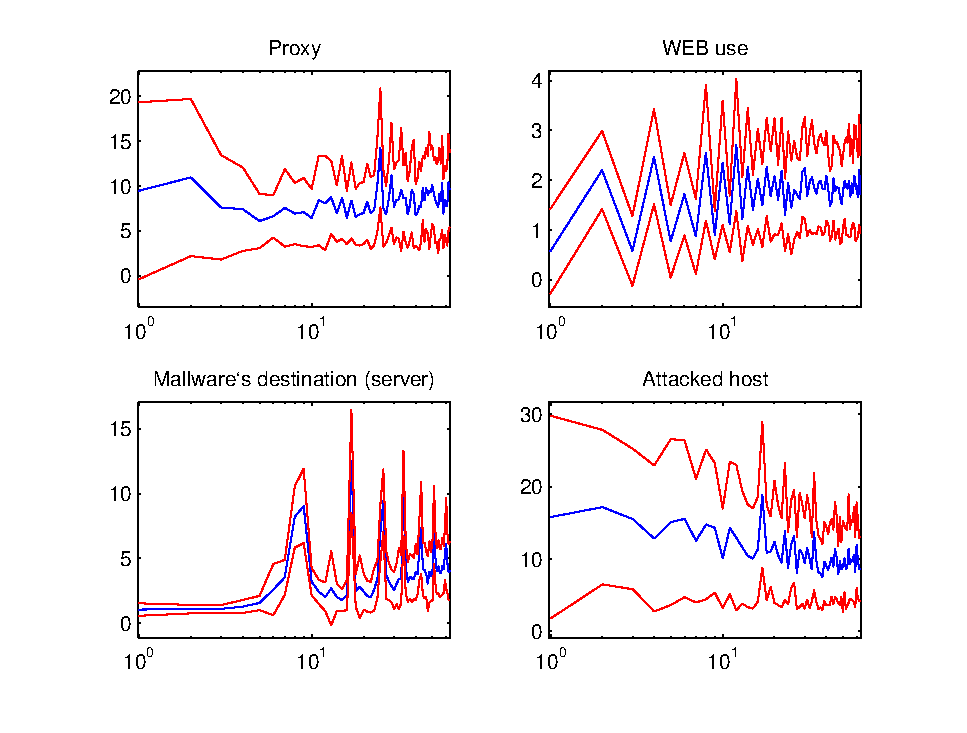
\includegraphics[width=140mm]{img/spect_dst_logp}
%  \caption{Spectrums ($mean$ - blue, $mean\pm st.dev$ - red) of some  endpoints using feature $r_t^{(2)}$ and agregation over \textbf{target}}
%  \label{fig:spect_dst_logp}
%\end{figure}
%\begin{figure}[h!]%
%  \centering
%  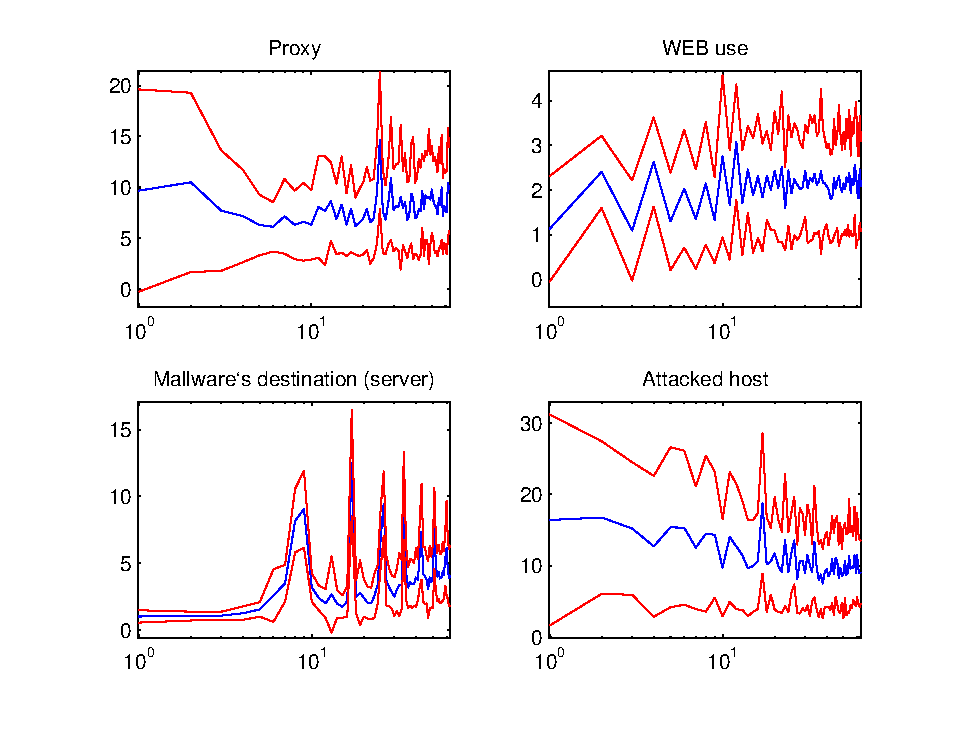
\includegraphics[width=140mm]{img/spect_src_logp}
%  \caption{Spectrums ($mean$ - blue, $mean\pm st.dev$ - red) of some  endpoints using feature $r_t^{(2)}$ and agregation over \textbf{source}}
%  \label{fig:spect_src_logp}
%\end{figure}
%\begin{figure}[h!]%
%  \centering
%  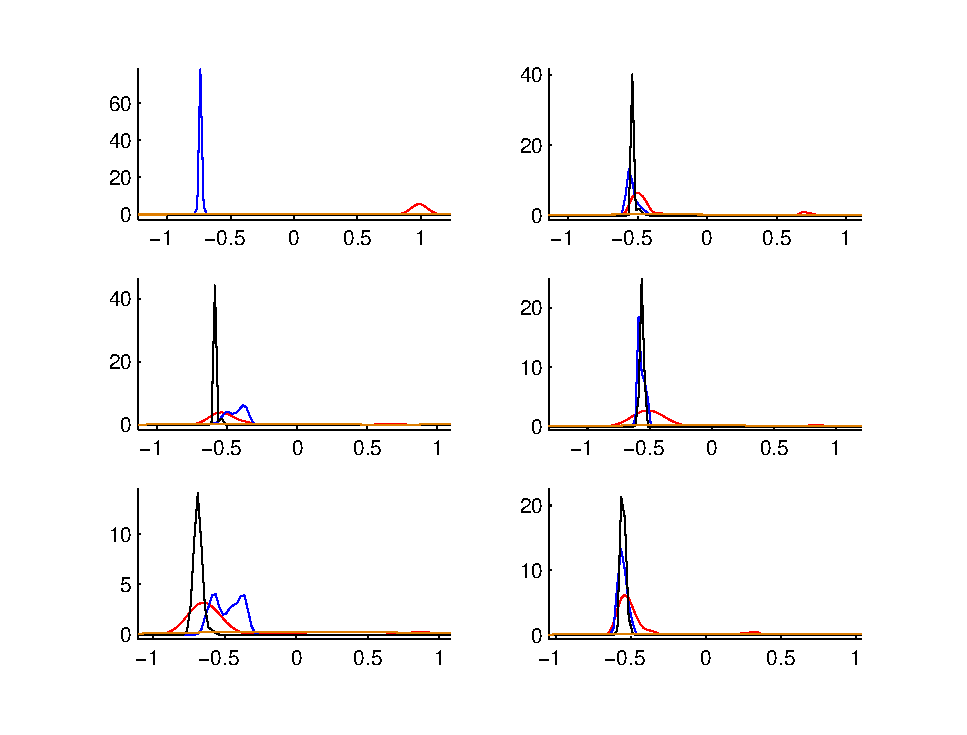
\includegraphics[width=140mm]{img/dens_dst_bdivp}
%      \includegraphics[width=40mm]{img/legend}
%  \caption{Conditional probability density estimation $Pr ( \mathcal{R}^{(1)}_{*,j}|_e ) $ using feature $r_t^{(1)}$ and agregation over \textbf{target}}
%  \label{fig:dens_dst_bdivp}
%\end{figure}
%\begin{figure}[h!]%
%  \centering
%  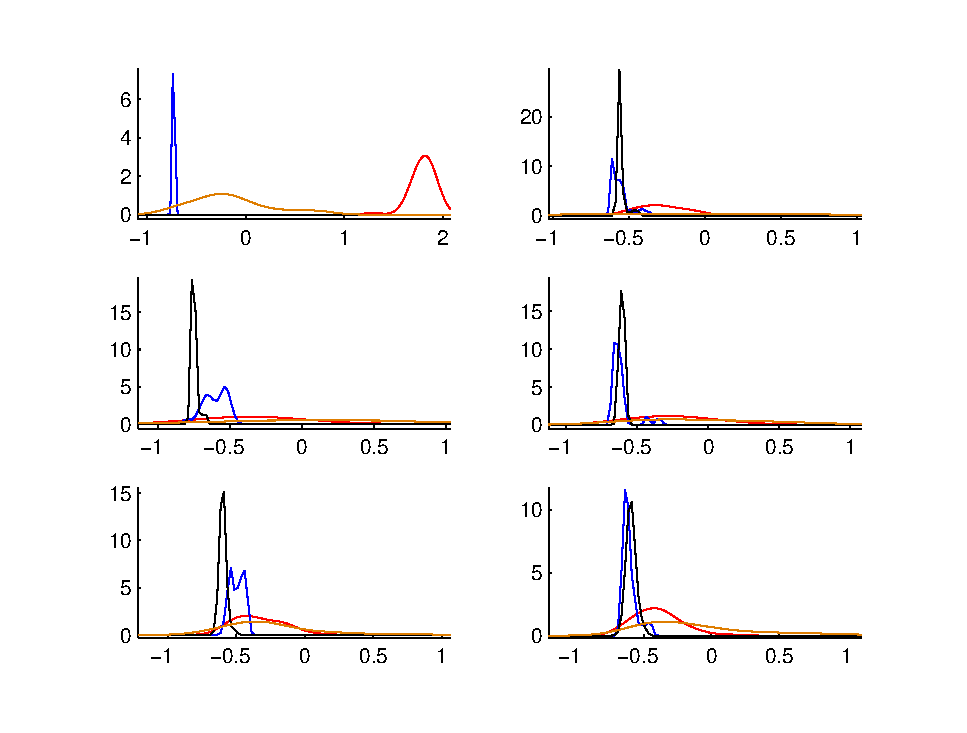
\includegraphics[width=140mm]{img/dens_src_bdivp}
%    \includegraphics[width=40mm]{img/legend}
%  \caption{Conditional probability density estimation $Pr ( \mathcal{R}^{(1)}_{*,j}|_e ) $ using feature $r_t^{(1)}$ and agregation over \textbf{source}}
%  \label{fig:dens_src_bdivp}
%\end{figure}
%\begin{figure}[h!]%
%  \centering
%  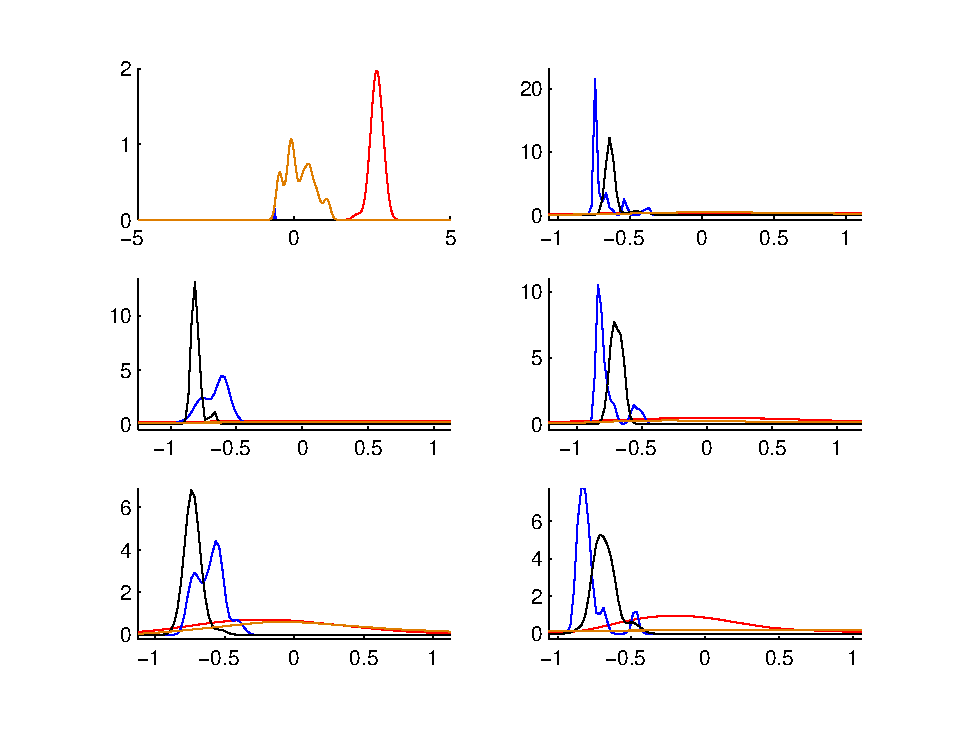
\includegraphics[width=140mm]{img/dens_dst_logp}
%      \includegraphics[width=40mm]{img/legend}
%  \caption{Conditional probability density estimation $Pr ( \mathcal{R}^{(2)}_{*,j}|_e ) $ using feature $r_t^{(2)}$ and agregation over \textbf{target}}
%  \label{fig:dens_dst_logp}
%\end{figure}
%\begin{figure}[h!]%
%  \centering
%  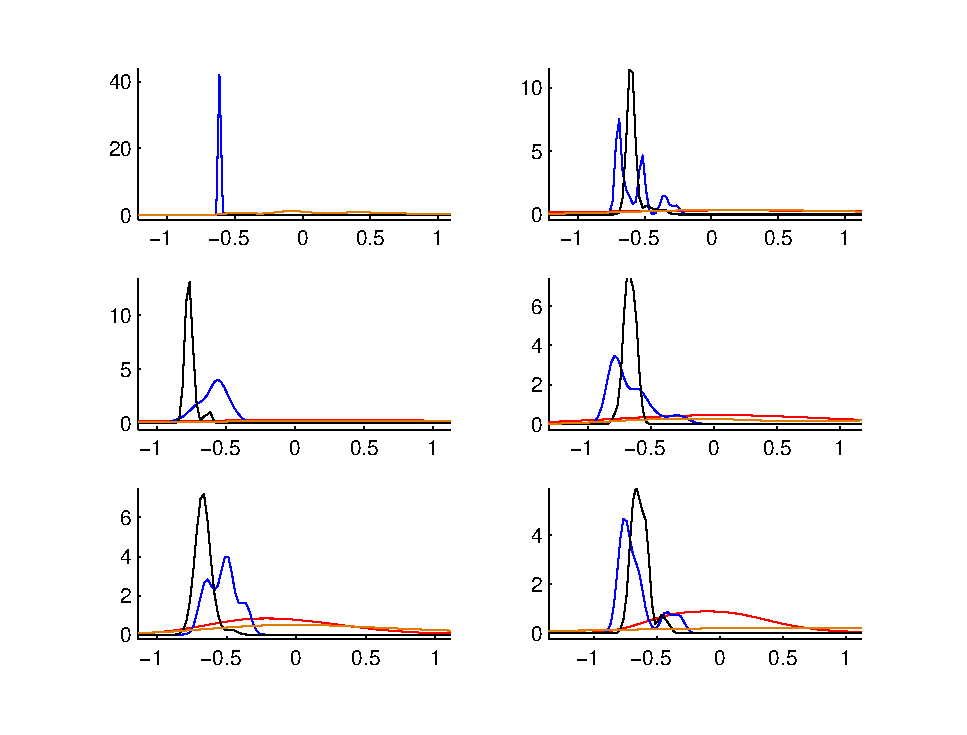
\includegraphics[width=140mm]{img/dens_src_logp}
%  \includegraphics[width=40mm]{img/legend}
%  \caption{Conditional probability density estimation $Pr ( \mathcal{R}^{(2)}_{*,j}|_e ) $ using feature $r_t^{(2)}$ and agregation over \textbf{source}}
%  \label{fig:dens_src_logp}
%\end{figure}
%\begin{figure}[h!]%
%  \centering
%  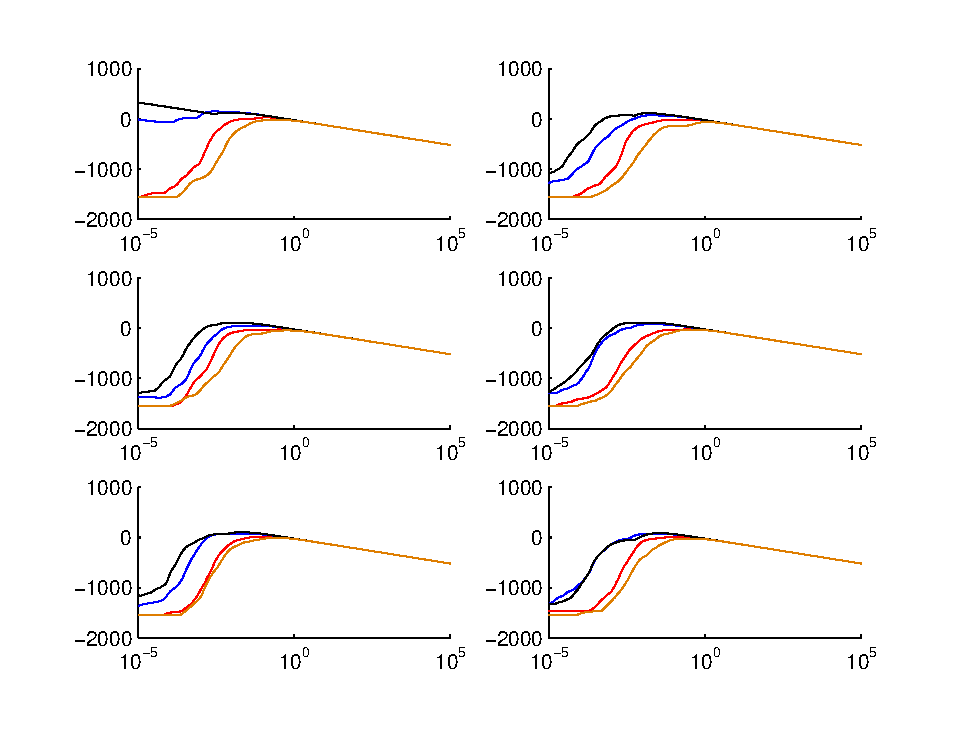
\includegraphics[width=140mm]{img/loglik_src_bdivp}
%  \includegraphics[width=40mm]{img/legend}
%  \caption{Example of log-likelihood functions $\log(L)$ used to estimate maximum likelihood}
%  \label{fig:loglik_src_bdivp}
%\end{figure}
%
